\section{Results}
\label{sec:results}

\subsection{System Objectives}
\label{sec:results:objectives}
Table~\ref{tab:objectives} reports every objective of
Section~\ref{sec:model} on the three deployments, and Fig.~\ref{fig:system}
shows the system costs behind O1, O1b and O4. All targets are met on VitalDB.
On WEAR all are met except the utility bound, which is inconclusive. On eICU
five of seven are met; the utility bound is inconclusive under the
prespecified interval criterion, with a point estimate above it, and is
missed end to end; update delivery falls short at two edges.

\begin{table}[!t]
\centering
\caption{Objectives, measured or simulated, against the targets fixed in advance}
\label{tab:objectives}
\small
\setlength{\tabcolsep}{3pt}
\begin{tabular}{llrrrl}
\toprule
& Quantity & VitalDB & WEAR & eICU & Target \\
\midrule
O1  & Uplink reduction     & $90.8\%$   & $96.1\%$   & $92.3\%$   & $\ge 50\%$ \\
O1b & Round latency cut    & $16.9\%$   & $21.7\%$   & $33.4\%$   & $> 0\%$ \\
O2a & Budget $\varepsilon$        & $0.900$    & $0.766^{\S}$ & $0.900$  & $\le 1$ \\
O2b & Utility loss [pts]   & $-1.18$    & $1.97$~pp$^{\dagger\S}$ & $3.10^{\dagger}$ & $\le 2$ \\
O3a & P95 latency [ms]     & $2.30$     & $0.75$     & $0.24$     & $< 100$ \\
O3b & Update delivery      & $100.00\%$ & $99.94\%$  & $97.83\%^{\ast}$ & $> 99\%$ \\
O4  & Energy saving        & $72.3\%$   & $76.8\%$   & $79.6\%$   & $\ge 20\%$ \\
\bottomrule
\end{tabular}
\tabnote{Measured: inference latency on a workstation CPU (ONNX Runtime) and the
uplink payload of the deployed update encoding. Simulated: delivery and round latency (packet-level ns-3, every
round) and energy (CloudSim Plus model). O2b: paired loss against an identical non-private system, five seeds,
in AUROC points. $^{\S}$Record-level; O2b is the accuracy loss over fifteen
seeds. $^{\dagger}$Interval spans the threshold (eICU: $[1.55, 4.65]$, point
estimate above it; end to end $3.88$ $[2.60, 5.17]$, not met). $^{\ast}$Not
met. VitalDB: O2a and O2b person-level, other rows
case-level. eICU: O2a and O2b with each person at one hospital, other rows on
the source partition (Section~\ref{sec:method:privacy}). O2a: training budget; the evaluated, non-deployed conformal
release adds $\varepsilon_{\mathrm{conf}} = 0.1$ on VitalDB and eICU (total
$1.0$) and $0.2$ on WEAR (total $0.966$).}
\end{table}

\begin{figure*}[!t]
\centering
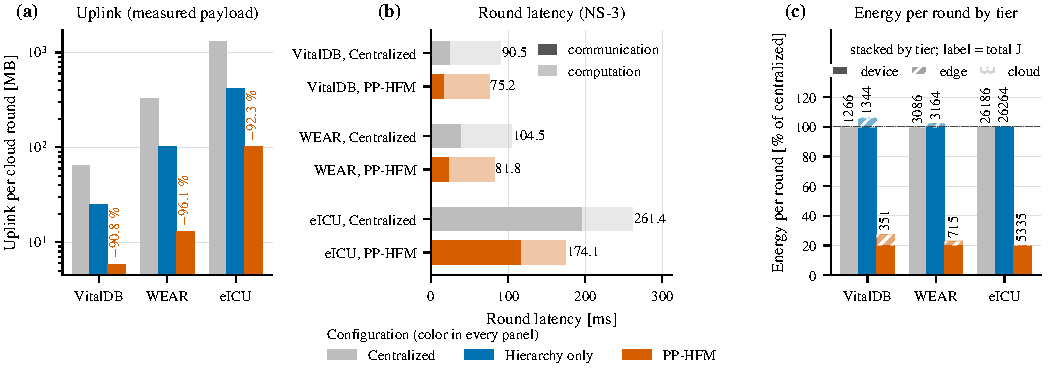
\includegraphics[width=\textwidth]{fig09_system_cost.pdf}
\caption{System cost: (a) uplink per cloud round, (b) round latency, (c) energy per round by tier, relative to centralized training.}
\label{fig:system}
\end{figure*}

\emph{Communication and latency.} Two-tier aggregation of the compressed head
update reduces uplink traffic by $90.8$, $96.1$ and $92.3\,\%$. The
measurement includes the index array that sparsification transmits with the
values, which analytical estimates omit. Round latency falls from $90.5$ to
$75.2$~ms on VitalDB, from $104.5$ to $81.8$~ms on WEAR and from $261.4$ to
$174.1$~ms on eICU, and the reduction is positive in every simulated round.
It is smaller than the traffic reduction because the hierarchy shortens link
time, not computation, and it grows with the number of stations sharing a
medium. Measuring every round at packet level matters: an earlier
configuration that composed nine rounds in ten analytically placed the
communication term of the centralized baseline at $256$~ms against $23.6$~ms
simulated, overstating the benefit fourfold.

\emph{Inference latency.} Timed on a workstation CPU (Intel Core i7-14700),
not on edge hardware, the $95$th-percentile latency is $2.30$, $0.75$ and
$0.24$~ms against a budget of $100$~ms (Table~\ref{tab:latency}). The private
mechanism adds no inference cost, because its noise acts only on training
gradients; eight-bit quantization was rejected because it raised the
$95$th percentile to $17.34$~ms.

\begin{table}[!t]
\centering
\caption{Inference latency on VitalDB ($1{,}000$ timed runs, workstation CPU)}
\label{tab:latency}
\small
\begin{tabular}{lrr}
\toprule
Stage & Mean [ms] & P95 [ms] \\
\midrule
Preprocessing              & $0.106$ & $0.110$ \\
Forward pass               & $2.130$ & $2.165$ \\
Conformal set (not deployed) & $0.019$ & $0.021$ \\
Post-processing            & $0.007$ & $0.008$ \\
\midrule
Total                      & $2.263$ & $2.299$ \\
Total, eight-bit graph     & $3.515$ & $17.337$ \\
\bottomrule
\end{tabular}
\tabnote{After $100$ warm-up runs. The eight-bit graph was evaluated and not
deployed.}
\end{table}

\emph{Reliability and energy.} Update delivery is $100.00$ and $99.94\,\%$ on
VitalDB and WEAR. On eICU, $187$ clients on two edges contend for the shared
medium, and delivery is $97.83\,\%$, against $95.11\,\%$ for centralized
training. With the edge count varied and everything else fixed, delivery
rises monotonically to $99.94\,\%$ at sixteen edges, meets the target on
average from six edges and in every round from eight (about $23$ clients per
edge, minimum $99.49\,\%$). Energy per round falls by $72.3$, $76.8$ and
$79.6\,\%$. Introducing the edge tier alone increases total energy, from
$1{,}266$ to $1{,}344$~J on VitalDB; the saving comes from the reduced device
computation and transmission of PP-HFM, which lowers the device term
fivefold.

\subsection{Privacy Budget and Utility}
\label{sec:results:privacy}
On both clinical corpora, the contribution to the training transcript of
every training patient is protected at
$\varepsilon = 0.900$, $\delta = 10^{-5}$, across all tiers; on eICU these runs
use the partition in which each person is held by one hospital
(Section~\ref{sec:method:privacy}). This is not an end-to-end guarantee for
the headline runs: their standardization constants are fitted on the
training cohort, and on VitalDB and WEAR the oracle encoders also violate
(A2) (Table~\ref{tab:ledger}). The VitalDB and WEAR results are therefore
comparisons of the private head, not end-to-end private deployments; the
only configuration that satisfies the guarantee end to end is the eICU rerun with disjoint encoders and pool-fitted constants, reported separately below. The per-client
multipliers range from $6.34$ to $15.56$ on VitalDB and from $4.85$ to
$29.34$ on eICU (median $13.76$); a single worst-case multiplier would have
imposed $29.34$ on every hospital.

\emph{A private calibration threshold.} A per-client conformal threshold
released by the exponential mechanism over ranks \cite{ref30, ref24}
($\varepsilon_{\mathrm{conf}} = 0.1$) was evaluated and is not part of the
system: with about a hundred calibration patients per client the private
threshold returns the majority-class set on every VitalDB seed and on four of
five eICU seeds, so coverage equals the base rate ($80.1\,\%$ on VitalDB,
case-level partition; $95.8\,\%$ on eICU) and misses the $90\,\%$ target.
The non-private threshold does not collapse (positive-class coverage
$36$--$43\,\%$), but its coverage, $80.4$--$81.8\,\%$, also misses the
target.

At the default threshold the private model predicts the majority class on
every VitalDB seed and on four of five eICU seeds (accuracy $0.8113$ and
$0.958$, the base rates), so accuracy measures the threshold rather than the model, and the
declared measures are used. On VitalDB the private model attains an AUROC of
$0.8318$ against $0.8200$ for the non-private reference, a change of $-1.18$
points $[-1.63, -0.73]$ ($p = 0.002$); AUPRC changes by $-3.47$
$[-6.33, -0.61]$ and balanced accuracy by $-0.31$ $[-1.23, +0.62]$, negative
values favoring the private model. O2b is met. The gain is consistent with
regularization of the compact head by clipping and noise, which the
case-level ablation suggests (Section~\ref{sec:results:ablation}) but this
experiment does not isolate; on the
case-level partition the change was $-0.90$ $[-1.82, +0.02]$. On eICU a cost is resolved: AUROC falls from
$0.8239$ to $0.7929$, by $3.10$ points $[1.55, 4.65]$; the interval spans the
two-point target, so O2b is inconclusive under the prespecified interval
criterion at five seeds, although the point estimate exceeds the target. AUPRC falls by $1.84$ $[1.60, 2.08]$, spanning the
threshold, and balanced accuracy by $0.33$ $[-0.22, +0.88]$, which meets it.
The cost is set by the smallest hospitals, which sample every patient at every
step and carry the largest multipliers. With standardization constants
fitted on the disjoint pool and encoders pretrained in those units, so that
the guarantee holds end to end, the eICU cost is $3.88$ points
$[2.60, 5.17]$, $2.31$ $[1.42, 3.21]$ in AUPRC and $2.80$ $[2.52, 3.08]$ in
balanced accuracy: O2b is missed in AUROC and in balanced accuracy, whose
intervals lie above the target, while the AUPRC interval spans it with a point
estimate above it. Assigning each person to one hospital left the cost of
privacy unchanged within resolution: against the same arms on the source
partition, paired by seed, the AUROC cost differs by $+0.01$ $[-0.72, +0.75]$
points with training-fitted and by $-0.03$ $[-0.66, +0.60]$ with pool-fitted
constants; on the source partition the end-to-end balanced-accuracy interval,
$[1.57, 3.82]$, had spanned the target. On WEAR, whose guarantee is
record-level, the accuracy loss is $1.97$ pp $[1.76, 2.17]$, spanning the
threshold.

\emph{Cost of the unit.} Moving the guarantee from the record to the patient
at a matched budget ($\varepsilon = 1$, five seeds, VitalDB) changes AUROC by
$-0.0170$ $[-0.0269, -0.0071]$ ($0.8423 \rightarrow 0.8254$) and AUPRC by
$-0.0582$ $[-0.0701, -0.0462]$ (case-level: $-0.0147$ and $-0.0783$). Two effects
contribute: sampling patients rather than records reduces the sampled units
from $33{,}491$ to $4{,}221$, and clipping a patient's summed gradient constrains
individuals with many records most. Section~\ref{sec:results:k} isolates the
second.

\emph{Cost of disjoint encoders.} With the disjoint instead of the oracle
encoders, the VitalDB model (case-level partition) loses $1.57 \pm 0.46$ AUROC points
($0.8395 \rightarrow 0.8237$, five paired seeds, $p < 0.001$) and
$1.22 \pm 2.62$ AUPRC points, which is not resolved. Against a non-private
reference with the same disjoint encoders, the cost of privacy is
$+0.14$ $[-0.33, +0.62]$ AUROC points, which meets O2b, and $+2.21$
$[-0.03, +4.46]$ AUPRC points.
This configuration satisfies (A2), but its standardization constants are still
fitted on the training individuals; on eICU, where the disjoint pool is not
carved from a small cohort, every result already uses disjoint encoders.

\subsection{Initialization, Not the Privatized Subset}
\label{sec:results:recipe}
PP-HFM differs from conventional private training in two respects: it starts
from pretrained encoders and privatizes only the head.
Table~\ref{tab:recipe} and Fig.~\ref{fig:recipe} separate the two. On VitalDB
(case-level partition), under the patient-level mechanism, changing only the initialization is worth
$0.0129$ AUROC without noise and $0.1991$ at $\varepsilon = 0.5$, increasing
monotonically as the budget tightens; on WEAR it ranges from $0.0021$ to
$0.3580$. Under privacy, restricting the privatized subset changes AUROC by
between $-0.0059$ and $-0.0025$ on VitalDB and by at most $0.0013$ on WEAR,
with intervals covering zero at every finite budget. Only without noise does
the head-only arm score higher on VitalDB, by $0.0139 \pm 0.0124$; no privacy
mechanism is involved there.

\begin{table}[!t]
\centering
\caption{Recipe decomposition in AUROC (three seeds; VitalDB case-level)}
\label{tab:recipe}
\setlength{\tabcolsep}{3.5pt}
\small
\begin{tabular}{lcccc}
\toprule
& \multicolumn{2}{c}{VitalDB} & \multicolumn{2}{c}{WEAR} \\
\cmidrule(lr){2-3}\cmidrule(lr){4-5}
$\varepsilon$ & B4$\rightarrow$B7 & B7$\rightarrow$B6 & B4$\rightarrow$B7 & B7$\rightarrow$B6 \\
\midrule
$\infty$ & $+0.0129$ & $+0.0139 \pm 0.0124$ & $+0.0021$ & $-0.0002 \pm 0.0003$ \\
$8$      & $+0.1407$ & $-0.0025 \pm 0.0059$ & $+0.0883$ & $+0.0001 \pm 0.0002$ \\
$4$      & $+0.1569$ & $-0.0029 \pm 0.0063$ & $+0.1257$ & $+0.0001 \pm 0.0002$ \\
$2$      & $+0.1727$ & $-0.0035 \pm 0.0040$ & $+0.1918$ & $+0.0002 \pm 0.0001$ \\
$1$      & $+0.1841$ & $-0.0059 \pm 0.0063$ & $+0.2827$ & $+0.0003 \pm 0.0008$ \\
$0.5$    & $+0.1991$ & $-0.0042 \pm 0.0043$ & $+0.3580$ & $+0.0013 \pm 0.0088$ \\
\bottomrule
\end{tabular}
\tabnote{B4$\rightarrow$B7 changes only the initialization; B7$\rightarrow$B6
only the privatized subset (whole network $\rightarrow$ head). Mean $\pm$
Student-$t$ half-width. VitalDB uses the patient-level mechanism on the
case-level partition; WEAR is record-level.}
\end{table}

\begin{figure*}[!t]
\centering
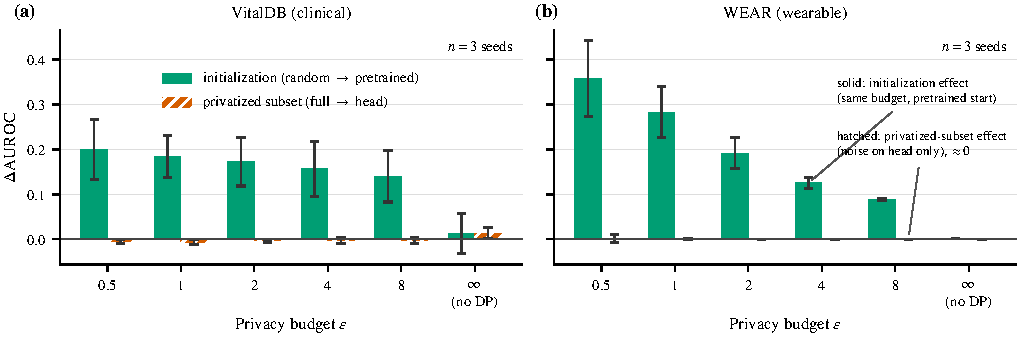
\includegraphics[width=\textwidth]{fig05_init_vs_subset.pdf}
\caption{Recipe decomposition across $\varepsilon$ (AUROC, $n = 3$, $95\,\%$ CI; VitalDB case-level): solid, initialization effect; hatched, privatized-subset effect.}
\label{fig:recipe}
\end{figure*}

The result contradicts a dimensionality explanation. If a smaller privatized
vector absorbed less noise, B7, which privatizes all $1{,}864{,}227$
parameters, should trail B6, which privatizes $559{,}874$, most at the
tightest budget. At $\varepsilon = 0.5$ the two differ by $0.0042$, within
the interval and with B7 the higher, consistent with the noise scale being set
by the budget, the step count and the sampling rate rather than by the number
of parameters. Across the budget range, the randomly initialized arm loses
$0.1906$ on VitalDB and $0.3716$ on WEAR, where it falls to $0.6247$, close to
chance; the pretrained full-model arm loses $0.0043$ and the head-only arm
$0.0225$ on VitalDB, and both less than $0.016$ on WEAR. Restricting the
subset is therefore justified by communication, since only the head is
transmitted, not by accuracy.

\subsection{Records per Individual}
\label{sec:results:k}
Table~\ref{tab:kscaling} and Fig.~\ref{fig:klaw} report the gap between the
record- and patient-level arms as the number of training records per
individual $k$ varies, with the units per step equal in both arms (VitalDB
case-level).

\begin{table}[!t]
\centering
\caption{AUPRC gap between the record and patient arms (three seeds; VitalDB case-level)}
\label{tab:kscaling}
\setlength{\tabcolsep}{3pt}
\small
\begin{tabular}{rcccc}
\toprule
& \multicolumn{2}{c}{VitalDB ($\varepsilon_{\mathrm{tr}} = 1$)} &
\multicolumn{2}{c}{eICU ($\varepsilon_{\mathrm{tr}} = 0.8$)} \\
\cmidrule(lr){2-3}\cmidrule(lr){4-5}
$k$ & Gap & $p$ & Gap & Forecast \\
\midrule
$1$  & $-0.0071 \pm 0.0599$ & $0.661$ & $-0.0011 \pm 0.0369$ & $0.0000$ \\
$2$  & $+0.0486 \pm 0.0129$ & $0.004$ & $+0.0048 \pm 0.0057$ & $0.0515$ \\
$4$  & $+0.0796 \pm 0.0163$ & $0.002$ & $+0.0081 \pm 0.0554$ & $0.0816$ \\
$8$  & $+0.0872 \pm 0.0248$ & $0.004$ & $+0.0099 \pm 0.0437$ & $0.0876$ \\
$16$ & --                   & --      & $+0.0103 \pm 0.0332$ & $0.0878$ \\
\bottomrule
\end{tabular}
\tabnote{Record arm minus patient arm, paired by seed; mean $\pm$ Student-$t$
half-width. The forecast for eICU was registered before the corpus was built.}
\end{table}

\begin{figure*}[!t]
\centering
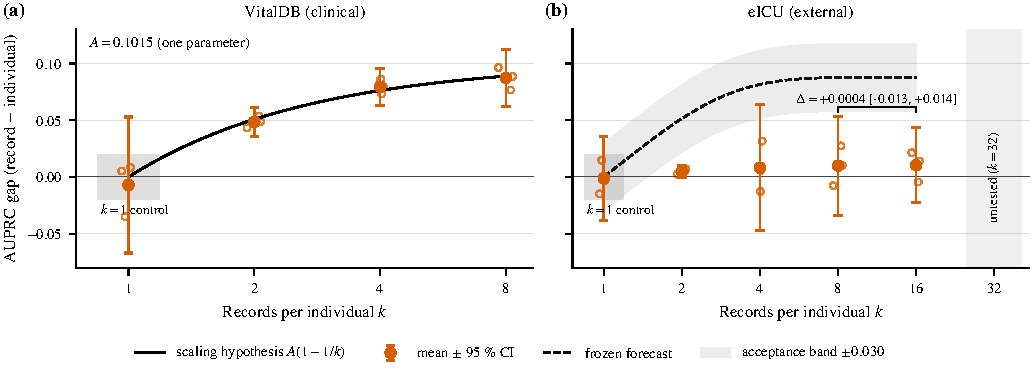
\includegraphics[width=\textwidth]{fig03_klaw.pdf}
\caption{Patient-level cost (AUPRC gap) against records per individual $k$, $n = 3$: (a) VitalDB (case-level) with the fitted curve $A(1-1/k)$; (b) eICU against the frozen forecast.}
\label{fig:klaw}
\end{figure*}

\emph{VitalDB.} At $k = 1$ the arms are indistinguishable ($-0.0071$, interval
covering zero), as Corollary~\ref{cor:k1} requires, so the divergence at
larger $k$ is attributable to the unit. From $k = 2$ the gap is resolved and
grows to $0.0872$ at $k = 8$. The patient-level arm is flat (means
$0.5083$--$0.5128$), whereas the record-level arm rises from $0.5015$ to
$0.5955$ (Fig.~\ref{fig:arms}): the widening gap is additional records that
the record-level arm exploits and the patient-level arm cannot, because the bound on the summed
contribution is tightest for the individuals who contribute them. AUROC moves
in the same direction ($+0.0026$ to $+0.0159$) but is unresolved at three
seeds.

\begin{figure}[!t]
\centering
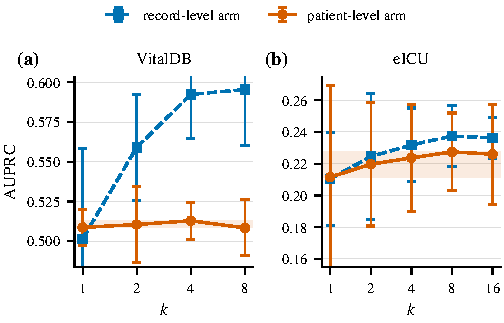
\includegraphics[width=\columnwidth]{fig04_arms.pdf}
\caption{AUPRC of each arm against $k$ ($n = 3$, $95\,\%$ CI): (a) VitalDB (case-level), where the patient-level arm is flat and the record-level arm improves; (b) eICU, where the arms overlap at every $k$.}
\label{fig:arms}
\end{figure}

\emph{Test of the scaling hypothesis.} The one-parameter curve
$A(1 - 1/k)$, fitted to the twelve paired gaps, gives $A = 0.1015$ at a
root-mean-square error of $0.0119$, against $0.0117$ for a two-parameter
saturating curve $A(1 - e^{-b(k-1)})$: the extra parameter buys nothing. Fitted
on $k \le 4$ only, it predicts $0.0904$ at $k = 8$ against $0.0872$ observed.
The patient-level arm changes by less than $0.001$ per doubling of $k$, as the
proposition requires.

\emph{External test on eICU.} Before the eICU corpus was built, a forecast was
registered from the VitalDB grid ($A = 0.0878$, $b = 0.883$) with an
acceptance band of $\pm 0.030$. On eICU the $k = 1$ control holds
($-0.0011$), and the ordering and the saturation reproduce: the gap
rises through $k = 8$ and changes by $+0.0004$
$[-0.0134, +0.0141]$ from $k = 8$ to $k = 16$, meeting the registered bound
on further growth. The magnitude does not: at $k = 8$ the gap is
$0.0099$, about one ninth of the forecast, and no eICU gap is resolved
at three seeds. Attainable precision differs by a factor of two between the
tasks (AUPRC near $0.22$ at a prevalence of $4.2\,\%$, against $0.5$), and a
cost that is a fixed fraction of attainable precision would preserve the
shape at a lower ceiling; distinguishing this from a corpus-specific ceiling
requires a third corpus. The registered design extended to $k = 32$, but only
$20.2\,\%$ of eICU individuals reach $32$ records, all of them readmitted, so
the maximum was reduced to $16$ by a dated amendment before any result beyond
$k = 8$ was computed.

\emph{Budget confound.} The forecast was fitted at
$\varepsilon = 1$ and tested at $0.8$ with a batch of $64$.
Re-running VitalDB at the eICU operating point (Table~\ref{tab:matched})
does not shrink its gaps ($+0.0914$ against $+0.0872$ at $k = 8$; the
one-parameter curve fitted on $k \le 4$ predicts $0.0988$), so the budget does
not explain the shortfall. That grid,
however, fails its own $k = 1$ control ($+0.0398$, all seeds of one sign),
which combines the smallest training pool with the largest batch; subtracting
each grid's $k = 1$ offset attributes about half ($51\,\%$) of the
difference at $k = 8$ to the operating point, and under neither reading does
the corpus term change sign.

\begin{table}[!t]
\centering
\caption{AUPRC gap across the three scaling grids (three seeds; VitalDB case-level)}
\label{tab:matched}
\setlength{\tabcolsep}{3.5pt}
\small
\begin{tabular}{ccccc}
\toprule
 & & \multicolumn{2}{c}{VitalDB} & eICU \\
\cmidrule(lr){3-4}\cmidrule(lr){5-5}
$k$ & Forecast & $\varepsilon_{\mathrm{tr}}\!=\!1.0$ & $\varepsilon_{\mathrm{tr}}\!=\!0.8$ & $\varepsilon_{\mathrm{tr}}\!=\!0.8$ \\
\midrule
$1$ & $0.0000$ & $-0.0071$ & $+0.0398$ & $-0.0011$ \\
$2$ & $0.0515$ & $+0.0486$ & $+0.0364$ & $+0.0048$ \\
$4$ & $0.0816$ & $+0.0796$ & $+0.0981$ & $+0.0081$ \\
$8$ & $0.0876$ & $+0.0872$ & $+0.0914$ & $+0.0099$ \\
\bottomrule
\end{tabular}
\tabnote{The two VitalDB grids differ only in the operating point. The forecast
was fitted on VitalDB at $\varepsilon_{\mathrm{tr}} = 1$ and never refitted.}
\end{table}

\emph{Clipping rule.} The flatness of the patient-level arm could stem from
the clipping rule rather than the unit. Normalizing each patient's summed
gradient by its record count, or its square root, before clipping leaves the
sensitivity and the budget unchanged and tests this. On the natural eICU
partition, where records per individual range from $2$ to $192$, the count
normalization lowers the final-round clipped fraction from $0.14$ to $0.08$
but changes AUPRC by $-0.0012$ $[-0.0093, +0.0069]$ (three seeds); the
one-sided $95\,\%$ upper bound, $+0.0043$, excludes the pre-registered
recovery of $+0.010$, and square-root normalization changes AUPRC by
$-0.0031$. On VitalDB at $k = 8$ and the same budget, count normalization
lowers the final-round clipped fraction from $0.50$ to $0.34$ and changes
AUPRC by $+0.0038$ $[-0.0072, +0.0148]$; the one-sided upper bound, $+0.0113$,
does not exclude $+0.010$, so this test is inconclusive by its own criterion,
and square-root normalization changes AUPRC by less than $10^{-4}$. The
clipping rule therefore does not explain the cost on eICU, and on VitalDB it
explains at most one eighth of the $0.0914$ cost at that operating point.

\subsection{Multimodal Fusion}
\label{sec:results:fusion}
On VitalDB (case-level partition) the fused model attains $0.8653 \pm 0.0072$ AUROC against
$0.8283 \pm 0.0087$ for the better single modality, a gain of $0.0370$ at
$5.9$ seed standard deviations, and $0.0671$ in AUPRC (five seeds). On WEAR
the better single modality already reaches $0.9976$, leaving no headroom. On
eICU fusion yields nothing in the natural configuration ($+0.0037$, and
$+0.0020$ on the partitions of the test below), where the admission stream
($0.8221$) dominates the vital-sign stream ($0.7068$). A
pre-registered test weakened the stronger stream to parity by mixing its
dominant feature with variance-preserving noise, calibrated on that stream
alone and never on the fused model (Table~\ref{tab:fusion},
Fig.~\ref{fig:fusion}). At parity the fused model exceeds the better single
modality by $0.0291 \pm 0.0211$, positive on all five seeds ($p = 0.019$),
fourteen times the matched control; the AUPRC gain, $0.0121 \pm 0.0215$, is
not resolved. Balance is therefore sufficient for a fusion gain on this
corpus, but not shown to be necessary, and the balanced model remains below
the intact admission stream. Because the eICU second stream is admission
data rather than a second sensor, this controlled test identifies a mechanism;
it does not show that a two-sensor clinical deployment would gain as much.

\begin{table}[!t]
\centering
\caption{Fusion on eICU as the stronger stream is weakened (AUROC, five
seeds; gains over the better single modality).}
\label{tab:fusion}
\setlength{\tabcolsep}{2.2pt}
\footnotesize
\begin{tabular}{lccccc}
\toprule
Condition & Vitals & Admission & Fused & Gain & Gain (AP) \\
\midrule
Matched control    & $0.7068$ & $0.8221$ & $0.8241$ & $+0.0020$ & $-0.0008$ \\
Feature zeroed     & $0.6973$ & $0.5947$ & $0.6911$ & $-0.0062$ & $-0.0182$ \\
Titrated to parity & $0.6992$ & $0.6845$ & $0.7282$ & $\mathbf{+0.0291}$ & $+0.0121$ \\
\bottomrule
\end{tabular}
\end{table}

\begin{figure}[!t]
\centering
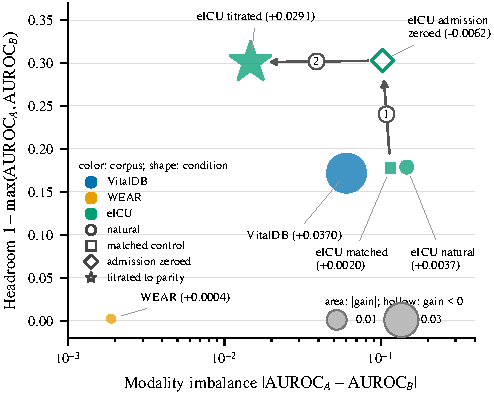
\includegraphics[width=\columnwidth]{fig06_fusion_map.pdf}
\caption{Fusion gain against modality imbalance and headroom (color: corpus; shape: condition; area: $|$gain$|$); numbered arrows trace the eICU titration.}
\label{fig:fusion}
\end{figure}

\subsection{Component Ablation and Membership-Inference Audit}
\label{sec:results:ablation}
Each component is removed in turn from the full system, three seeds paired
(case-level)
(Table~\ref{tab:ablation}, Fig.~\ref{fig:audit}(a)). Removing sparsification
($+0.0012$) or quantization ($+0.0001$, the narrowest interval in the study)
leaves accuracy unchanged and raises uplink fivefold and $1.6$-fold, so
compression is justified by traffic alone. Removing the edge tier costs
$-0.0058$ at three seeds and is resolved at the six pre-registered seeds,
$-0.0047$ $[-0.0088, -0.0006]$ on VitalDB and $-0.0052$
$[-0.0074, -0.0030]$ on WEAR; because the flat arm also changes the
aggregation schedule, this bounds the cost of the hierarchy rather than
claiming a benefit. Removing the privacy mechanism \emph{reduces} AUROC by
$0.0234$: two of three non-private seeds peak in the first round and then
degrade, whereas every private seed peaks between rounds six and nine, so
clipping and noise regularize a compact head over frozen features. The
loss-aware edge weighting of an earlier version (C6) adds nothing and is not
adopted.

\begin{table}[!t]
\centering
\caption{Component ablation on VitalDB (record-level mechanism, case-level partition, three seeds)}
\label{tab:ablation}
\small
\setlength{\tabcolsep}{4pt}
\begin{tabular}{llcr}
\toprule
Removed & AUROC & $\Delta$AUROC & MB \\
\midrule
--- (full)        & $0.8541$ & ---                  & $252$ \\
C1 hierarchy      & $0.8484$ & $-0.0058 \pm 0.0088$ & $50$ \\
C2 privacy        & $0.8307$ & $\mathbf{-0.0234 \pm 0.0205}$ & $252$ \\
C3 sparsification & $0.8553$ & $+0.0012 \pm 0.0083$ & $1260$ \\
C4 quantization   & $0.8543$ & $+0.0001 \pm 0.0006$ & $403$ \\
+C6 loss weighting & $0.8542$ & $+0.0001 \pm 0.0009$ & $252$ \\
\bottomrule
\end{tabular}
\tabnote{$\Delta$AUROC is paired against the full system; bold: the interval
excludes zero. MB: total uplink. C6 is an inclusion arm.}
\end{table}

\begin{figure*}[!t]
\centering
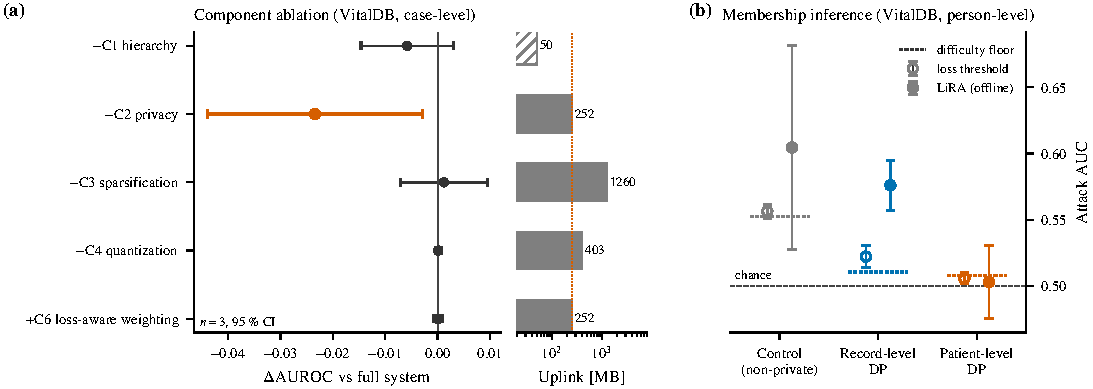
\includegraphics[width=\textwidth]{fig10_ablation_mia.pdf}
\caption{VitalDB: (a) component ablation, case-level ($\Delta$AUROC, $n = 3$, $95\,\%$ CI); (b) membership inference, person-level, against each difficulty floor (dotted).}
\label{fig:audit}
\end{figure*}

\emph{Audit.} Table~\ref{tab:mia} reports the leakage of three
configurations on the person-level partition. The positive control,
non-private training of the same head, shows that the audit detects
leakage: offline LiRA reaches $0.605$, $0.052$ above its difficulty floor and
$0.048$ above the loss threshold, and online LiRA with a global variance
reaches $0.597$ $[0.586, 0.609]$, entirely above the floor; at three seeds the
offline interval spans the floor. Record-level training remains detectably
above its floor under offline LiRA ($0.576$, margin $+0.065$), whereas
patient-level training does not ($0.503$, margin $-0.005$). The record-level
arm is not equivalent to the control: it lies below it under the loss
threshold ($0.522$ against $0.556$) and online LiRA with a global variance
($0.508$ against $0.597$), and the two were not compared statistically (three
control seeds against five). The attack that validates the control (online,
global variance) is thus not the one that separates the two units (offline).
Paired over five seeds on identical shadow
splits, the record-level arm exceeds the patient-level arm by $+0.073$
$[0.054, 0.092]$ ($p < 0.001$) for offline LiRA and by $+0.016$
$[0.010, 0.023]$ ($p = 0.002$) for the loss threshold, both surviving
correction for four attacks; the two online attacks resolve no difference.
The direction is as predicted, but the magnitude is smaller: the record-level
attack reaches $0.576$, not the predicted $0.7$. On the case-level partition,
where members were operations, no difference was resolved ($+0.029$
$[-0.038, +0.095]$ for offline LiRA). The audit covers VitalDB only and
bounds what these attacks achieve; it does not establish the absence of
leakage.

\begin{table}[!t]
\centering
\caption{Membership inference on VitalDB (person-level partition)}
\label{tab:mia}
\small
\setlength{\tabcolsep}{2.5pt}
\begin{tabular}{lccc}
\toprule
Configuration & Loss AUC & LiRA AUC & Floor \\
\midrule
Control (no DP) & $0.556$ {\scriptsize$[0.551, 0.561]$} & $0.605$ {\scriptsize$[0.528, 0.681]$} & $0.553$ \\
Record-level DP & $0.522$ {\scriptsize$[0.514, 0.531]$} & $0.576$ {\scriptsize$[0.557, 0.594]$} & $0.511$ \\
Patient-level DP & $0.506$ {\scriptsize$[0.502, 0.510]$} & $0.503$ {\scriptsize$[0.475, 0.531]$} & $0.508$ \\
\bottomrule
\end{tabular}
\tabnote{Mean attack AUC with $95\,\%$ interval over the target seeds (three
for the control, five otherwise); LiRA is the offline likelihood-ratio attack.
Floor: the AUC from per-patient difficulty alone, without the target model.}
\end{table}

\emph{Attribution.} Integrated gradients over $512$ test windows (case-level)
give the
$22$ missingness indicators $15.8\,\%$ of the prediction without privacy and
$21.6$--$21.7\,\%$ under either unit with frozen encoders, below their
$42\,\%$ share of inputs.

\subsection{Comparison with Prior Systems}
\label{sec:results:prior}
HED-FL \cite{ref3} and FL2DP \cite{ref9} were re-implemented and trained
through the same trainer, splits, frozen encoders, rounds and five seeds as
PP-HFM (Table~\ref{tab:prior}). HED-FL aggregates hierarchically without
privacy, uploads dense updates and samples $60\,\%$ of the clients per round;
FL2DP perturbs every coordinate with an exponential mechanism and shuffles the
updates, without a hierarchy. FL2DP was run on VitalDB only, because its
per-coordinate mechanism would take about two GPU days per seed on eICU.

\emph{Utility and traffic.} On VitalDB, PP-HFM exceeds FL2DP by $0.0123$
AUROC $[0.0064, 0.0181]$ and $0.025$ AUPRC $[0.015, 0.035]$, and HED-FL by
$0.030$ AUPRC $[0.005, 0.055]$; the AUROC difference from HED-FL, $0.0056$
$[-0.0018, +0.0131]$, is not resolved. HED-FL exceeds the non-private PP-HFM
reference by $0.0062$ AUROC $[0.0011, 0.0113]$.
On eICU, HED-FL is $3.17$ AUROC points $[1.56, 4.77]$ and $1.77$ AUPRC points
$[0.75, 2.78]$ above the private model and level with the non-private
reference ($+0.0008$, $p = 0.39$), so the gap is the price of the
patient-level guarantee measured in Section~\ref{sec:results:privacy}. PP-HFM
uploads $2.2$ times less than HED-FL on VitalDB, $2.4$ times less on eICU, and
$4.0$ times less than FL2DP.

\emph{Leakage.} On VitalDB, under the audit of
Section~\ref{sec:results:ablation}, on the same seeds and shadow splits, offline LiRA reaches $0.581$ against HED-FL
and $0.608$ against FL2DP, $0.078$ $[0.050, 0.106]$ and $0.105$
$[0.079, 0.130]$ above PP-HFM; the loss threshold gives $+0.047$ and
$+0.055$. Both baselines also have higher difficulty floors ($0.555$ and
$0.559$ against $0.508$), and their margins above them are $+0.026$ and
$+0.049$, against $-0.005$ for PP-HFM. The PP-HFM is the patient-level audit target, trained at $\varepsilon = 1.0$ with $\varepsilon_{\mathrm{conf}} = 0.5$ and one worst-client multiplier under the R\'enyi accountant, not the $\varepsilon = 0.9$ model whose AUROC and uplink are listed, so its leakage is measured at a slightly weaker budget than the headline. The comparison bounds what these attacks achieve and does not by itself establish the guarantee. FL2DP leaks more than HED-FL, which adds no noise at all.
Its candidate set is built from the private gradient value
(Eqs.~11--12 of \cite{ref9}), so the mechanism satisfies no finite
$\varepsilon$, and the audit finds that it does not reduce leakage either.

\begin{table}[!t]
\centering
\caption{PP-HFM against re-implemented prior systems (five seeds)}
\label{tab:prior}
\small
\setlength{\tabcolsep}{3pt}
\begin{tabular}{llcccc}
\toprule
& System & $\varepsilon$ & AUROC & MB & LiRA \\
\midrule
\multirow{3}{*}{\rotatebox{90}{\scriptsize VitalDB}}
& PP-HFM & $0.90$ & $\mathbf{0.8318}$ & $\mathbf{252}$ & $\mathbf{0.503}$ {\scriptsize$(-0.005)$} \\
& HED-FL & $\infty$ & $0.8262$ & $560$ & $0.581$ {\scriptsize$(+0.026)$} \\
& FL2DP & --- & $0.8195$ & $1008$ & $0.608$ {\scriptsize$(+0.049)$} \\
\midrule
\multirow{2}{*}{\rotatebox{90}{\scriptsize eICU}}
& PP-HFM & $0.90$ & $0.7936$ & $\mathbf{5235}$ & --- \\
& HED-FL & $\infty$ & $\mathbf{0.8252}$ & $12541$ & --- \\
\bottomrule
\end{tabular}
\tabnote{$\varepsilon$: patient-level training budget ($\delta = 10^{-5}$);
---: no finite bound. MB: total uplink. LiRA: offline attack AUC,
margin above the difficulty floor in parentheses; not run on eICU. The
PP-HFM LiRA entry is the patient-level audit target (Section~\ref{sec:method:mia}:
$\varepsilon = 1.0$, $\varepsilon_{\mathrm{conf}} = 0.5$, one worst-client
multiplier, R\'enyi accountant), not the $\varepsilon = 0.9$ model whose AUROC
and uplink are listed. eICU rows: source partition, on which the baselines
were run ($2.9\,\%$ of training persons at several hospitals,
Section~\ref{sec:method:privacy}). All AUROC
differences from PP-HFM are resolved except HED-FL on VitalDB.}
\end{table}
